% !TEX program = xelatex
% =====================================================================
%  赛道二·方向1B｜科研影响力分析与偏差解释 —— 提交要求及模板（LaTeX 版）
%  编译方式：XeLaTeX 编译两到三遍，使目录与页码稳定（见文末说明）。
%  源文件：《赛道二-方向1B-科研影响力分析与偏差解释-提交要求及模板.docx》
% =====================================================================
\documentclass[letterpaper]{ctexart}

% ---------- 页面：Letter 纸张，四周约 1 英寸 ----------
\usepackage[letterpaper,margin=1in,headheight=14pt,headsep=12pt,footskip=26pt]{geometry}

% ---------- 图形 / 颜色 ----------
\usepackage{graphicx}
\graphicspath{{fig/}}
\usepackage[table]{xcolor}
\definecolor{shadegray}{gray}{0.93}   % 表头底纹（很浅的灰）
\definecolor{notebg}{gray}{0.96}      % 提示框底纹（更浅的灰）

% ---------- 表格 ----------
\usepackage{array}
\usepackage{longtable}

% ---------- 页眉页脚 ----------
\usepackage{fancyhdr}

% ---------- 提示框 / 备注框 ----------
\usepackage{tcolorbox}

% ---------- 超链接：黑色、无边框 ----------
\usepackage[hidelinks]{hyperref}
\hypersetup{pdftitle={方向 1B｜科研影响力分析与偏差解释——提交要求及模板}}

% ---------- 字号、行距、段距 ----------
\linespread{1.3}\selectfont
\setlength{\parindent}{0pt}
\setlength{\parskip}{0.55em}

% ---------- 标题：黑色黑体，章节顺序即原文 P1—P20 ----------
\setcounter{secnumdepth}{0}      % 标题文字自带 P1｜… 编号，不另加自动编号
\setcounter{tocdepth}{2}         % 目录显示到二级标题
\ctexset{
  section = {
    format      = {\zihao{-3}\bfseries\heiti},
    beforeskip  = 0.5em,
    afterskip   = 1em,
  },
  subsection = {
    format      = {\zihao{4}\bfseries\heiti},
    beforeskip  = 1.2em,
    afterskip   = 0.7em,
  },
}

% ---------- 页眉页脚：全部页面（含首页与目录页）统一 ----------
\newcommand{\headertext}{面向上海城市户外运动的多源环境暴露感知与健康路线决策 AI Scientist}
\pagestyle{fancy}
\fancyhf{}
\fancyhead[L]{\small\headertext}
\fancyfoot[R]{\small 赛道二·数据场景 · \thepage}
\renewcommand{\headrulewidth}{0.4pt}
\fancypagestyle{plain}{%
  \fancyhf{}
  \fancyhead[L]{\small\headertext}
  \fancyfoot[R]{\small 赛道二·数据场景 · \thepage}
  \renewcommand{\headrulewidth}{0.4pt}
}

% ---------- 提示框（由原文单格说明表转换而来） ----------
\newtcolorbox{notebox}{
  colback = notebg,
  colframe = black,
  boxrule = 0.5pt,
  arc = 0pt,
  boxsep = 2pt,
  left = 6pt, right = 6pt, top = 4pt, bottom = 4pt,
}

% ---------- 表格辅助命令 ----------
\newcommand{\thead}[1]{\textbf{#1}}                       % 表头：黑色加粗
\newcommand{\colw}[1]{\dimexpr#1\textwidth-2\tabcolsep-2\arrayrulewidth\relax}
\newcolumntype{\cw}[1]{>{\raggedright\arraybackslash}p{\colw{#1}}}  % 按比例定宽、自动换行列
\newcommand{\tcell}{\rule{0pt}{2.6em}}                    % 空白行的最小行高（只抬高、不截断）

% ---------- 填写区：整洁横线，保留可继续填写的空白 ----------
\newcommand{\fillin}[1]{\par\noindent #1\hrulefill\par}   % 题干 + 横线
\newcommand{\fillblank}{\par\noindent \hrulefill\par}     % 整行横线

\begin{document}

% =====================================================================
% 开头标题信息
% =====================================================================
\begin{center}
    {\zihao{-3}\bfseries\heiti 2026年度中国青年科技创新“揭榜挂帅”擂台赛 · 阿里云榜题}\\[8pt]
    {\zihao{-2}\bfseries\heiti 方向 1B｜科研影响力分析与偏差解释}\\[8pt]
    {\zihao{5}\bfseries 赛道二·数据场景｜题目编号：XH-202619｜依据：阿里云赛事官网}
\end{center}
\vspace{0.8em}

% 原首页页眉中的“使用说明”，按要求转为正文提示框保留
\begin{notebox}
    使用说明：本模板仅供技术报告的结构与论证参考，无需逐页对应，也不要求写满20页；团队可根据作品实际调整章节和篇幅，但技术方案PPT/PDF仍须符合官网“不超过20页”的要求。较长代码、运行日志、完整数据清单和分析结果等可按赛事允许形式另附，并在正文中说明对应关系；最终以官网及提交系统最新要求为准。
\end{notebox}

% =====================================================================
% 目录（由真实章节结构自动生成，页码与链接由 LaTeX 维护）
% =====================================================================
\clearpage
\tableofcontents
\clearpage

% =====================================================================
% P1｜作品信息与核心结果
% =====================================================================
\section{P1｜作品信息与核心结果}

\subsection{参赛团队信息/成员信息（必须将盖章版本的报名表第一页和第二页截图贴上来）}

\begin{center}
    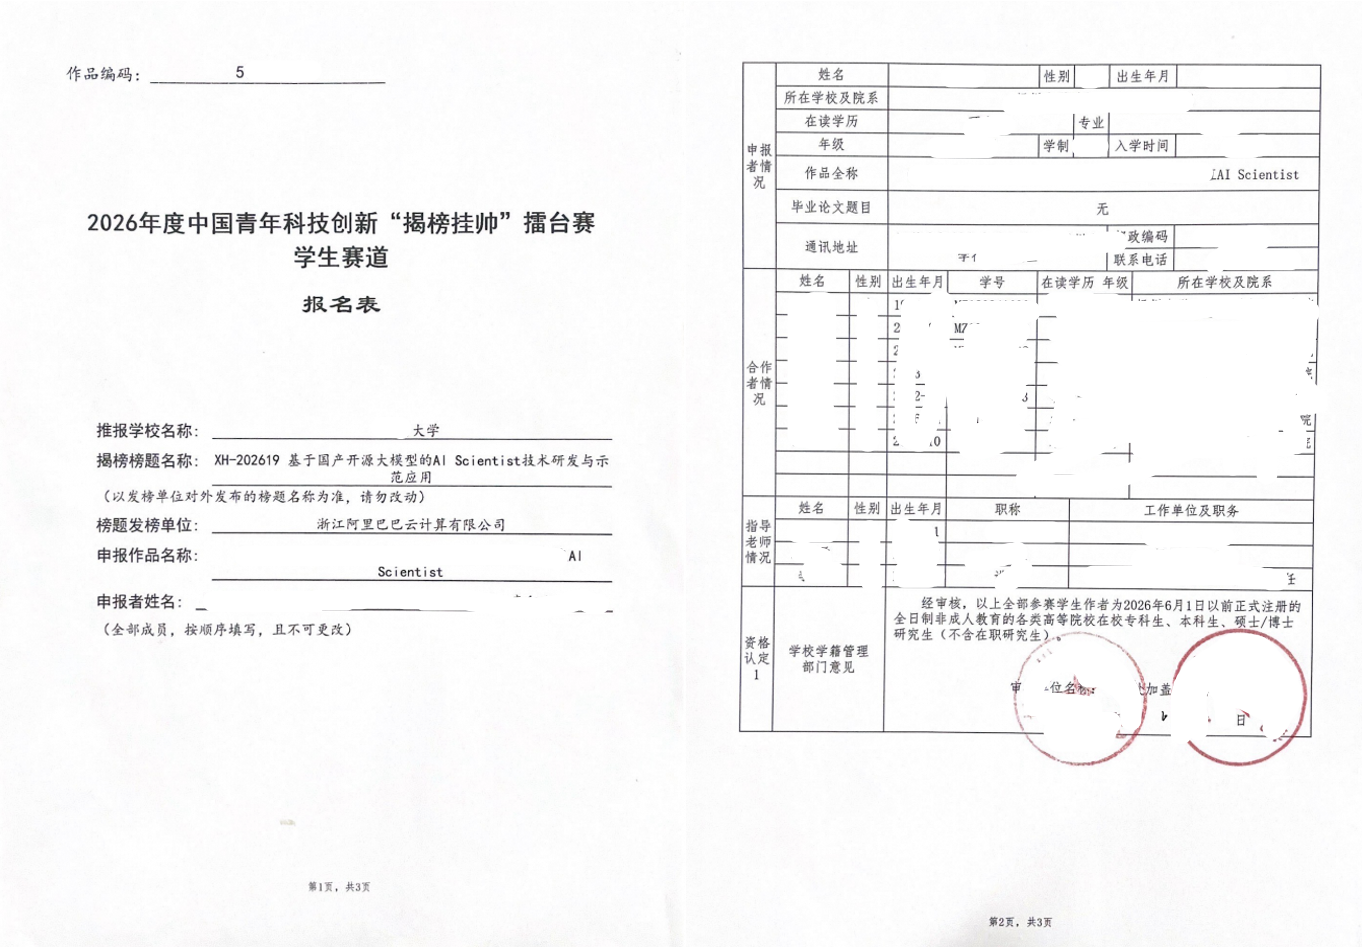
\includegraphics[width=0.92\textwidth]{image1.png}
\end{center}

\subsection{作品基本信息}

{\setlength{\tabcolsep}{5pt}\renewcommand{\arraystretch}{1.3}
    \begin{longtable}{|\cw{0.34}|\cw{0.66}|}
        \hline
        \thead{挑战杯系统报名时参赛作品名称（必填）}                            & xxxxxxxxxxxxxxxxxxxxxxxx  \\ \hline
        \thead{最终参赛作品名称（如有更新可备注）}                             & xxxxxxxxxxxxxxxxxxxxxxxxx \\ \hline
        \thead{参赛选题（必填-赛道几第几个方向选题）}                           & 如赛道一-选题1-A                \\ \hline
        \thead{参赛作品简介（300字内）-（必填）}                            & xxxxxxxxxxxxxxxxxxxxxxxx  \\ \hline
        \thead{参赛作品使用Qwen大模型及AI技术说明（300字内）-（必填）}              & xxxxxxxxxxxxxxxxxxxxxxxx  \\ \hline
        \thead{宣传视频链接/其他作品相关文件（没有的可忽略）链接 / 视频需上传至夸克网盘，分享链接复制} & xxxxxxxxxxxxxxxxxxxxxxxx  \\ \hline
    \end{longtable}}

\subsection{本作品核心主张}

\fillin{本作品实际分析的对象与用途：}
\fillin{本作品对“影响力”的实际定义：}
\fillin{最有代表性的结果1（任务范围、方法、结果）：}
\fillin{最有代表性的结果2（偏差或不稳定问题、证据、结论）：}
\fillin{目前仍存在的主要局限：}

\subsection{官网要求提示}

技术方案文档PPT/PDF不超过20页，应包含研究问题与解决方法、架构设计与讲解、代表性测试案例、源代码、项目工作流程、上下文工程设计、数据或资料来源说明、结果展示与反馈迭代过程等内容。

基座模型须使用Qwen系列，并通过阿里云百炼或官网推荐工具调用，提供调用凭证或截图。

本方向重点展示对论文、研究方向或学术成果的影响力分析，以及影响因素、可能偏差和不稳定性的解释；不能只给出一个缺少依据的分数。

如提供可交互前端、测试API或10分钟以内演示视频，应保证展示内容与正文和代码一致。

% =====================================================================
% P2｜作品目标与实际完成内容
% =====================================================================
\clearpage
\section{P2｜作品目标与实际完成内容}

\subsection{团队实际解决的问题}

{\small [请用一段话说明：现有科研评价或文献分析方式在什么场景下存在什么具体不足，本作品希望帮助谁解决其中哪一项问题。不要重复赛事背景。]}

\fillblank

\subsection{本作品实际完成的工作}

{\small [请用一段话概括已经实现的功能，例如输入解析、信息提取、影响力判断、主要因素解释、偏差或不稳定性识别、人工复核或反馈修正；没有实现的内容不必写。]}

\fillblank

\subsection{本作品形成的完整分析过程}

{\small [请插入总体思路图，建议呈现：分析对象与目的 → 数据和资料获取 → 内容解析 → 影响力判断 → 主要因素解释 → 偏差检查 → 质量核验或人工反馈 → 结果与边界。]}

\fillin{本作品最终给出的分析结果形式：}
\fillin{本作品已经实际处理的对象和任务范围：}
\fillin{相较简单指标、人工整理或通用模型直接回答，本作品最主要的不同：}

% =====================================================================
% P3｜本作品所说的“影响力”是什么
% =====================================================================
\clearpage
\section{P3｜本作品所说的“影响力”是什么}

\subsection{请按本作品实际定义填写}

{\setlength{\tabcolsep}{5pt}\renewcommand{\arraystretch}{1.3}
    \begin{longtable}{|\cw{0.34}|\cw{0.66}|}
        \hline
        \rowcolor{shadegray} \thead{要回答的问题} & \thead{团队实际填写内容} \\ \hline
        \endfirsthead
        \hline
        \rowcolor{shadegray} \thead{要回答的问题} & \thead{团队实际填写内容} \\ \hline
        \endhead
        \tcell 本作品分析什么对象                    &                  \\ \hline
        \tcell 谁会使用分析结果，用于什么任务              &                  \\ \hline
        \tcell 本作品所说的“影响力”具体指什么             &                  \\ \hline
        \tcell 最终输出分数、等级、排序、因素分析还是其他结论      &                  \\ \hline
        \tcell 该结果不能说明什么，也不能用于什么决定          &                  \\ \hline
    \end{longtable}}

\subsection{使用边界}

\fillin{分析所依据的数据时间范围或截止时间：}
\fillin{影响力判断适用于哪些对象、领域或条件：}
\fillin{是否涉及论文质量、研究价值或未来表现；如涉及，依据和限制是什么：}
\fillin{必须由研究者或人工复核的内容：}

\begin{notebox}
    “影响力”不等于“科学质量”，也不应自动成为评价个人、团队或研究成果的唯一依据。作品可以输出分数，也可以输出等级、排序、因素分析或带条件的判断。
\end{notebox}

% =====================================================================
% P4｜本作品实际使用的数据与资料
% =====================================================================
\clearpage
\section{P4｜本作品实际使用的数据与资料}

\subsection{已实际使用的来源}

{\setlength{\tabcolsep}{5pt}\renewcommand{\arraystretch}{1.3}
    \begin{longtable}{|\cw{0.18}|\cw{0.22}|\cw{0.22}|\cw{0.17}|\cw{0.21}|}
        \hline
        \rowcolor{shadegray} \thead{数据或资料来源} & \thead{实际获取的内容} & \thead{版本、时间范围或截止时间} & \thead{为什么使用} & \thead{缺失与已知局限} \\ \hline
        \endfirsthead
        \hline
        \rowcolor{shadegray} \thead{数据或资料来源} & \thead{实际获取的内容} & \thead{版本、时间范围或截止时间} & \thead{为什么使用} & \thead{缺失与已知局限} \\ \hline
        \endhead
        \tcell                               &                 &                      &               &                 \\ \hline
        \tcell                               &                 &                      &               &                 \\ \hline
        \tcell                               &                 &                      &               &                 \\ \hline
        \tcell                               &                 &                      &               &                 \\ \hline
    \end{longtable}}

\subsection{来源和证据说明}

\fillin{团队实际使用了哪些论文内容、作者或期刊信息、引用关系、主题资料、开放数据或其他来源：}
\fillin{不同来源之间有哪些覆盖、重复、缺失或冲突：}
\fillin{输出中如何区分原始资料、规则计算、模型判断和人工意见：}
\fillin{无法核实、无权使用或不适合纳入分析的内容如何处理：}

\begin{notebox}
    只填写实际使用的来源。来源越多不一定越好，关键是说明它与分析目标的关系、截止时间和已知缺口。
\end{notebox}

% =====================================================================
% P5｜验证方案与成功标准
% =====================================================================
\clearpage
\section{P5｜验证方案与成功标准}

\subsection{团队准备怎样验证作品}

{\setlength{\tabcolsep}{5pt}\renewcommand{\arraystretch}{1.3}
    \begin{longtable}{|\cw{0.18}|\cw{0.20}|\cw{0.22}|\cw{0.18}|\cw{0.22}|}
        \hline
        \rowcolor{shadegray} \thead{要验证的问题} & \thead{准备采用的判断方法} & \thead{使用哪些测试对象或样本} & \thead{什么情况算通过} & \thead{什么情况算失败或无法判断} \\ \hline
        \endfirsthead
        \hline
        \rowcolor{shadegray} \thead{要验证的问题} & \thead{准备采用的判断方法} & \thead{使用哪些测试对象或样本} & \thead{什么情况算通过} & \thead{什么情况算失败或无法判断} \\ \hline
        \endhead
        \tcell 影响力结果是否合理                    &                   &                     &                 &                      \\ \hline
        \tcell 主要因素解释是否有依据                  &                   &                     &                 &                      \\ \hline
        \tcell 偏差提示是否具体                     &                   &                     &                 &                      \\ \hline
        \tcell 结果是否稳定、可复核或可复现               &                   &                     &                 &                      \\ \hline
    \end{longtable}}

\subsection{验证原则}

\fillin{测试对象或样本如何选取，能否覆盖作品主要任务：}
\fillin{由什么参考结果、专家判断、公开信息或对照方法进行核验：}
\fillin{团队最重视哪几项检查，为什么：}
\fillin{哪些结果必须判为错误、无法判断或需要人工复核：}

\begin{notebox}
    本页只说明“准备用什么标准检验作品”，不填写最终结果。实际测试范围和结果分别在P14—P16展示；不要求所有作品采用同一种指标。
\end{notebox}

% =====================================================================
% P6｜系统总体架构与完整分析过程
% =====================================================================
\clearpage
\section{P6｜系统总体架构与完整分析过程}

\subsection{本作品真实架构}

{\small [请插入本作品实际架构图，标明分析对象、原始资料、提取信息、影响力结果、因素解释、偏差提示和质量反馈的流动方向，以及Qwen、外部工具和人工参与的位置。]}

{\setlength{\tabcolsep}{5pt}\renewcommand{\arraystretch}{1.3}
    \begin{longtable}{|\cw{0.17}|\cw{0.14}|\cw{0.29}|\cw{0.14}|\cw{0.26}|}
        \hline
        \rowcolor{shadegray} \thead{实际环节} & \thead{输入} & \thead{本作品实际怎么处理} & \thead{输出} & \thead{出错或无法判断时怎么做} \\ \hline
        \endfirsthead
        \hline
        \rowcolor{shadegray} \thead{实际环节} & \thead{输入} & \thead{本作品实际怎么处理} & \thead{输出} & \thead{出错或无法判断时怎么做} \\ \hline
        \endhead
        \tcell 输入理解与内容解析                  &            &                   &            &                     \\ \hline
        \tcell 数据和资料获取                    &            &                   &            &                     \\ \hline
        \tcell 影响力分析                      &            &                   &            &                     \\ \hline
        \tcell 因素解释与偏差检查                  &            &                   &            &                     \\ \hline
        \tcell 质量核验与结果输出                  &            &                   &            &                     \\ \hline
    \end{longtable}}

\subsection{完整过程说明}

{\small [请沿着一项真实任务说明：输入如何进入系统，结果如何形成，证据和限制如何附在结果中；如作品实际采用反馈或迭代，再说明问题如何返回前面的环节。]}

% =====================================================================
% P7｜Qwen使用方式与上下文工程
% =====================================================================
\clearpage
\section{P7｜Qwen使用方式与上下文工程}

\subsection{Qwen在本作品中的实际作用}

{\setlength{\tabcolsep}{5pt}\renewcommand{\arraystretch}{1.3}
    \begin{longtable}{|\cw{0.32}|\cw{0.68}|}
        \hline
        \rowcolor{shadegray} \thead{要说明的内容} & \thead{本作品实际做法} \\ \hline
        \endfirsthead
        \hline
        \rowcolor{shadegray} \thead{要说明的内容} & \thead{本作品实际做法} \\ \hline
        \endhead
        \tcell 使用的Qwen模型与调用方式               &                 \\ \hline
        \tcell Qwen实际承担哪些任务                 &                 \\ \hline
        \tcell 一次分析时实际提供给模型的内容              &                 \\ \hline
        \tcell 要求模型按照什么结构输出                 &                 \\ \hline
        \tcell Qwen与检索、数据库、代码或其他工具如何配合      &                 \\ \hline
    \end{longtable}}

\subsection{一次真实上下文示例}

{\small [请展示一次真实分析请求的结构，可包括分析目的、输入内容、可用资料、判断规则、历史结果或反馈、期望输出格式；删除密钥和个人信息。]}

\fillin{团队为减少无依据判断、错误归因或过度结论采取了什么措施：}
\fillin{不同来源、不同时间的资料如何进入上下文：}
\fillin{该设计对实际分析结果带来了什么变化：}

% =====================================================================
% P8｜输入解析与信息提取
% =====================================================================
\clearpage
\section{P8｜输入解析与信息提取}

\subsection{本作品实际处理的输入}

{\setlength{\tabcolsep}{5pt}\renewcommand{\arraystretch}{1.3}
    \begin{longtable}{|\cw{0.16}|\cw{0.24}|\cw{0.18}|\cw{0.16}|\cw{0.26}|}
        \hline
        \rowcolor{shadegray} \thead{实际输入类型} & \thead{提取了什么内容} & \thead{使用什么方法} & \thead{如何核对} & \thead{无法获取或无法确认时怎么做} \\ \hline
        \endfirsthead
        \hline
        \rowcolor{shadegray} \thead{实际输入类型} & \thead{提取了什么内容} & \thead{使用什么方法} & \thead{如何核对} & \thead{无法获取或无法确认时怎么做} \\ \hline
        \endhead
        \tcell                              &                 &                &              &                       \\ \hline
        \tcell                              &                 &                &              &                       \\ \hline
        \tcell                              &                 &                &              &                       \\ \hline
        \tcell                              &                 &                &              &                       \\ \hline
    \end{longtable}}

\subsection{一项真实提取示例}

{\small [请选择一篇论文、一项研究成果、一组文献或一个研究方向，展示原始输入、实际提取内容和核对结果。只填写本作品真实处理的内容。]}

\fillblank

\begin{notebox}
    输入可以是论文，也可以是研究方向、学术成果或其他实际分析对象；不要求所有作品同时处理题目、摘要、正文、作者、期刊、参考文献、引用关系和开放数据。
\end{notebox}

% =====================================================================
% P9｜影响力分析的核心方法
% =====================================================================
\clearpage
\section{P9｜影响力分析的核心方法}

\subsection{从判断依据到结果的实际过程}

{\setlength{\tabcolsep}{5pt}\renewcommand{\arraystretch}{1.3}
    \begin{longtable}{|\cw{0.18}|\cw{0.24}|\cw{0.17}|\cw{0.21}|\cw{0.20}|}
        \hline
        \rowcolor{shadegray} \thead{实际使用的依据} & \thead{为什么与P3定义的影响力相关} & \thead{系统如何使用} & \thead{形成什么中间或最终结果} & \thead{可能带来的局限或偏差} \\ \hline
        \endfirsthead
        \hline
        \rowcolor{shadegray} \thead{实际使用的依据} & \thead{为什么与P3定义的影响力相关} & \thead{系统如何使用} & \thead{形成什么中间或最终结果} & \thead{可能带来的局限或偏差} \\ \hline
        \endhead
        \tcell                               &                        &                &                     &                    \\ \hline
        \tcell                               &                        &                &                     &                    \\ \hline
        \tcell                               &                        &                &                     &                    \\ \hline
        \tcell                               &                        &                &                     &                    \\ \hline
    \end{longtable}}

\subsection{方法说明}

\fillin{本作品采用模型训练、微调、智能体、规则计算、工具调用还是组合方法：}
\fillin{从输入到最终结论依次经过哪些关键步骤：}
\fillin{哪些信息真正参与判断，哪些仅作为背景或展示：}
\fillin{数据缺失、时间滞后或信息冲突时，系统如何处理：}
\fillin{如输出分数、等级或排序，其含义和形成方法是什么：}

\begin{notebox}
    本页同时说明“依据什么”和“怎样形成结果”，不要求采用固定特征或固定技术路线，也不把引用次数、期刊或作者信息天然视为科学质量。
\end{notebox}

% =====================================================================
% P10｜结果表达与证据解释
% =====================================================================
\clearpage
\section{P10｜结果表达与证据解释}

\subsection{系统实际输出什么}

{\setlength{\tabcolsep}{5pt}\renewcommand{\arraystretch}{1.3}
    \begin{longtable}{|\cw{0.20}|\cw{0.24}|\cw{0.20}|\cw{0.16}|\cw{0.20}|}
        \hline
        \rowcolor{shadegray} \thead{输出内容或结论} & \thead{对应的实际证据} & \thead{系统如何解释} & \thead{应如何理解} & \thead{不能说明什么} \\ \hline
        \endfirsthead
        \hline
        \rowcolor{shadegray} \thead{输出内容或结论} & \thead{对应的实际证据} & \thead{系统如何解释} & \thead{应如何理解} & \thead{不能说明什么} \\ \hline
        \endhead
        \tcell                               &                 &                &               &                \\ \hline
        \tcell                               &                 &                &               &                \\ \hline
        \tcell                               &                 &                &               &                \\ \hline
    \end{longtable}}

\subsection{解释如何形成和核对}

\fillin{主要因素由模型、规则、统计方法、工具还是人工判断得到：}
\fillin{团队如何核对解释与原始资料、分析过程和最终结论是否一致：}
\fillin{同一结果存在多种解释时，系统如何呈现：}
\fillin{哪些内容属于原始事实、计算结果、相关线索或模型推断：}
\fillin{哪些表述不能写成因果结论：}

\begin{notebox}
    解释应能回到具体资料和分析步骤，不能用听起来合理但没有证据的文字代替分析。
\end{notebox}

% =====================================================================
% P11｜偏差、不公平与结果不稳定性
% =====================================================================
\clearpage
\section{P11｜偏差、不公平与结果不稳定性}

\subsection{本作品实际检查的方法}

{\setlength{\tabcolsep}{5pt}\renewcommand{\arraystretch}{1.3}
    \begin{longtable}{|\cw{0.16}|\cw{0.20}|\cw{0.18}|\cw{0.24}|\cw{0.22}|}
        \hline
        \rowcolor{shadegray} \thead{检查的问题} & \thead{为什么需要检查} & \thead{系统如何发现} & \thead{可能影响哪些对象或结果} & \thead{如何处理或提示} \\ \hline
        \endfirsthead
        \hline
        \rowcolor{shadegray} \thead{检查的问题} & \thead{为什么需要检查} & \thead{系统如何发现} & \thead{可能影响哪些对象或结果} & \thead{如何处理或提示} \\ \hline
        \endhead
        \tcell                             &                 &                &                     &                 \\ \hline
        \tcell                             &                 &                &                     &                 \\ \hline
        \tcell                             &                 &                &                     &                 \\ \hline
        \tcell                             &                 &                &                     &                 \\ \hline
    \end{longtable}}

\subsection{判断边界}

\fillin{如何区分偏差、正常差异和暂时无法判断：}
\fillin{如何说明受影响的对象、范围或程度：}
\fillin{哪些问题需要人工复核或补充数据：}
\fillin{哪些偏差或不稳定性当前无法可靠识别：}

\begin{notebox}
    可按作品实际检查数据覆盖、领域、语言、时间以及对作者、机构或期刊信息的依赖，不要求全部采用。偏差提示应具体到对象、数据或判断环节。
\end{notebox}

% =====================================================================
% P12｜质量控制、异常处理与人工介入
% =====================================================================
\clearpage
\section{P12｜质量控制、异常处理与人工介入}

\subsection{系统怎样避免把不可靠结果直接交给用户}

{\setlength{\tabcolsep}{5pt}\renewcommand{\arraystretch}{1.3}
    \begin{longtable}{|\cw{0.20}|\cw{0.20}|\cw{0.20}|\cw{0.16}|\cw{0.24}|}
        \hline
        \rowcolor{shadegray} \thead{可能出现的问题} & \thead{系统如何发现} & \thead{自动处理方式} & \thead{何时转人工} & \thead{最终如何标记或输出} \\ \hline
        \endfirsthead
        \hline
        \rowcolor{shadegray} \thead{可能出现的问题} & \thead{系统如何发现} & \thead{自动处理方式} & \thead{何时转人工} & \thead{最终如何标记或输出} \\ \hline
        \endhead
        \tcell                               &                &                &               &                   \\ \hline
        \tcell                               &                &                &               &                   \\ \hline
        \tcell                               &                &                &               &                   \\ \hline
    \end{longtable}}

\subsection{实际控制方式}

\fillin{哪些环节设置了资料核对、规则检查、模型复核或人工审核：}
\fillin{哪些情况下系统选择拒绝回答、降低结论强度或提示证据不足：}
\fillin{人工可以修改什么，不能修改什么，修改是否留有记录：}
\fillin{团队如何防止错误资料、单一指标或模型臆测主导最终结论：}

% =====================================================================
% P13｜代表性案例的完整分析过程
% =====================================================================
\clearpage
\section{P13｜代表性案例的完整分析过程}

\subsection{案例选择}

\fillin{案例对应的真实任务及选择理由：}
\fillin{本案例能够展示的关键能力：}
\fillin{本案例没有覆盖的任务或条件：}

\subsection{从输入到结论}

{\setlength{\tabcolsep}{5pt}\renewcommand{\arraystretch}{1.3}
    \begin{longtable}{|\cw{0.14}|\cw{0.26}|\cw{0.20}|\cw{0.18}|\cw{0.22}|}
        \hline
        \rowcolor{shadegray} \thead{分析环节} & \thead{本案例的实际输入或资料} & \thead{系统实际处理} & \thead{得到的结果} & \thead{对应证据与人工参与} \\ \hline
        \endfirsthead
        \hline
        \rowcolor{shadegray} \thead{分析环节} & \thead{本案例的实际输入或资料} & \thead{系统实际处理} & \thead{得到的结果} & \thead{对应证据与人工参与} \\ \hline
        \endhead
        \tcell 输入与资料获取                    &                     &                &               &                   \\ \hline
        \tcell 信息提取与核对                    &                     &                &               &                   \\ \hline
        \tcell 影响力分析                      &                     &                &               &                   \\ \hline
        \tcell 因素与偏差解释                    &                     &                &               &                   \\ \hline
        \tcell 质量核验与输出                    &                     &                &               &                   \\ \hline
    \end{longtable}}

\begin{notebox}
    用一个真实案例把完整过程讲清楚即可，不再把案例输入、结果和解释拆成三页。案例既要呈现有效结果，也要保留缺失、错误或需要人工确认的内容。
\end{notebox}

% =====================================================================
% P14｜实际测试任务与样本覆盖
% =====================================================================
\clearpage
\section{P14｜实际测试任务与样本覆盖}

\subsection{团队实际测试了什么}

{\setlength{\tabcolsep}{5pt}\renewcommand{\arraystretch}{1.3}
    \begin{longtable}{|\cw{0.20}|\cw{0.12}|\cw{0.16}|\cw{0.28}|\cw{0.24}|}
        \hline
        \rowcolor{shadegray} \thead{测试任务或对象类型} & \thead{实际数量} & \thead{选择方式} & \thead{覆盖的领域、时间或其他差异} & \thead{对应P5中的验证目标} \\ \hline
        \endfirsthead
        \hline
        \rowcolor{shadegray} \thead{测试任务或对象类型} & \thead{实际数量} & \thead{选择方式} & \thead{覆盖的领域、时间或其他差异} & \thead{对应P5中的验证目标} \\ \hline
        \endhead
        \tcell                                 &              &              &                       &                    \\ \hline
        \tcell                                 &              &              &                       &                    \\ \hline
        \tcell                                 &              &              &                       &                    \\ \hline
        \tcell                                 &              &              &                       &                    \\ \hline
    \end{longtable}}

\fillin{测试内容是否覆盖作品声称支持的主要任务：}
\fillin{是否包含普通案例、困难案例、资料缺失案例或容易产生偏差的案例：}
\fillin{哪些对象未纳入测试，为什么：}
\fillin{测试数据、资料截止时间和实际结果文件的位置：}

\begin{notebox}
    本页回答“实际测了什么”，不重复说明算法或逐项展开代表性案例。
\end{notebox}

% =====================================================================
% P15｜总体测试结果
% =====================================================================
\clearpage
\section{P15｜总体测试结果}

\subsection{按P5设定的标准汇总结果}

{\setlength{\tabcolsep}{5pt}\renewcommand{\arraystretch}{1.3}
    \begin{longtable}{|\cw{0.18}|\cw{0.20}|\cw{0.22}|\cw{0.18}|\cw{0.22}|}
        \hline
        \rowcolor{shadegray} \thead{验证目标} & \thead{实际测试范围} & \thead{实际结果} & \thead{是否达到团队标准} & \thead{证据或结果位置} \\ \hline
        \endfirsthead
        \hline
        \rowcolor{shadegray} \thead{验证目标} & \thead{实际测试范围} & \thead{实际结果} & \thead{是否达到团队标准} & \thead{证据或结果位置} \\ \hline
        \endhead
        \tcell 影响力结果合理性                   &                &              &                  &                 \\ \hline
        \tcell 主要因素解释                     &                &              &                  &                 \\ \hline
        \tcell 偏差提示具体程度                   &                &              &                  &                 \\ \hline
        \tcell 稳定性、可复核或可复现性               &                &              &                  &                 \\ \hline
    \end{longtable}}

\fillin{最能支持本作品核心主张的总体结果：}
\fillin{未达到预期的结果：}
\fillin{定量结果、人工判断和案例观察是否一致：}
\fillin{团队认为结果优越性的证据是什么，而不仅是主观判断：}

% =====================================================================
% P16｜异常、偏差与稳定性测试结果
% =====================================================================
\clearpage
\section{P16｜异常、偏差与稳定性测试结果}

\subsection{实际发现了什么}

{\setlength{\tabcolsep}{5pt}\renewcommand{\arraystretch}{1.3}
    \begin{longtable}{|\cw{0.20}|\cw{0.22}|\cw{0.17}|\cw{0.18}|\cw{0.23}|}
        \hline
        \rowcolor{shadegray} \thead{测试条件或异常情况} & \thead{结果发生了什么变化} & \thead{是否影响主要结论} & \thead{原因分析} & \thead{当前处理或提示方式} \\ \hline
        \endfirsthead
        \hline
        \rowcolor{shadegray} \thead{测试条件或异常情况} & \thead{结果发生了什么变化} & \thead{是否影响主要结论} & \thead{原因分析} & \thead{当前处理或提示方式} \\ \hline
        \endhead
        \tcell                                 &                   &                  &              &                   \\ \hline
        \tcell                                 &                   &                  &              &                   \\ \hline
        \tcell                                 &                   &                  &              &                   \\ \hline
    \end{longtable}}

\fillin{实际发现的主要偏差或不稳定问题：}
\fillin{哪些条件变化不会明显改变结论：}
\fillin{哪些情况下结果明显变差、失效或无法判断：}
\fillin{这些结果是否与P11中的偏差检查方法一致：}

\begin{notebox}
    只展示团队真实完成的检查结果；没有做过的压力测试或条件变化实验不必补写。
\end{notebox}

% =====================================================================
% P17｜人工复核、反馈与修正记录（如实际发生）
% =====================================================================
\clearpage
\section{P17｜人工复核、反馈与修正记录（如实际发生）}

\subsection{实际记录}

{\setlength{\tabcolsep}{5pt}\renewcommand{\arraystretch}{1.3}
    \begin{longtable}{|\cw{0.16}|\cw{0.28}|\cw{0.14}|\cw{0.20}|\cw{0.22}|}
        \hline
        \rowcolor{shadegray} \thead{发生在哪个环节} & \thead{实际发现的问题或收到的反馈} & \thead{如何复核} & \thead{实际采取的处理} & \thead{当前结论或仍存问题} \\ \hline
        \endfirsthead
        \hline
        \rowcolor{shadegray} \thead{发生在哪个环节} & \thead{实际发现的问题或收到的反馈} & \thead{如何复核} & \thead{实际采取的处理} & \thead{当前结论或仍存问题} \\ \hline
        \endhead
        \tcell                               &                       &              &                 &                   \\ \hline
        \tcell                               &                       &              &                 &                   \\ \hline
        \tcell                               &                       &              &                 &                   \\ \hline
    \end{longtable}}

\fillin{哪类问题可以由系统自动处理：}
\fillin{哪类问题需要研究者或其他人员确认：}
\fillin{反馈是否改变了资料、规则、提示、模型使用方式或最终表述：}
\fillin{实际处理带来了什么改善、代价或新问题：}

\begin{notebox}
    本页只填写作品开发或测试中真实发生的复核、反馈和修正。没有相关记录可不展开，不要求构造版本对照。
\end{notebox}

% =====================================================================
% P18｜对照结果与方案优越性
% =====================================================================
\clearpage
\section{P18｜对照结果与方案优越性}

\subsection{团队真实完成的比较}

{\setlength{\tabcolsep}{5pt}\renewcommand{\arraystretch}{1.3}
    \begin{longtable}{|\cw{0.15}|\cw{0.21}|\cw{0.14}|\cw{0.16}|\cw{0.15}|\cw{0.19}|}
        \hline
        \rowcolor{shadegray} \thead{实际比较对象} & \thead{保持相同的输入与资料条件} & \thead{检查方法} & \thead{本作品结果} & \thead{对照结果} & \thead{结论与代价} \\ \hline
        \endfirsthead
        \hline
        \rowcolor{shadegray} \thead{实际比较对象} & \thead{保持相同的输入与资料条件} & \thead{检查方法} & \thead{本作品结果} & \thead{对照结果} & \thead{结论与代价} \\ \hline
        \endhead
        \tcell                              &                      &              &               &              &               \\ \hline
        \tcell                              &                      &              &               &              &               \\ \hline
        \tcell                              &                      &              &               &              &               \\ \hline
    \end{longtable}}

\subsection{从三个层面说明优越性}

\fillin{科学逻辑：影响力定义、证据关系或结论边界实际改善了什么：}
\fillin{技术实现：输入处理、分析方法、解释、偏差检查或质量控制改善了什么：}
\fillin{结果表现：在哪些测试、案例或评价标准上取得了更好结果：}
\fillin{代价与不足：没有改善什么，增加了哪些数据、时间、调用或人工成本：}

\begin{notebox}
    可以与简单指标、人工判断、通用模型、其他方法或去掉关键环节后的版本比较，但只能填写团队真实完成的对照。
\end{notebox}

% =====================================================================
% P19｜失败案例、局限与适用边界
% =====================================================================
\clearpage
\section{P19｜失败案例、局限与适用边界}

\subsection{真实失败或边界问题}

{\setlength{\tabcolsep}{5pt}\renewcommand{\arraystretch}{1.3}
    \begin{longtable}{|\cw{0.20}|\cw{0.24}|\cw{0.20}|\cw{0.18}|\cw{0.18}|}
        \hline
        \rowcolor{shadegray} \thead{失败或边界问题} & \thead{实际表现} & \thead{原因分析} & \thead{当前处理方式} & \thead{是否影响核心结论} \\ \hline
        \endfirsthead
        \hline
        \rowcolor{shadegray} \thead{失败或边界问题} & \thead{实际表现} & \thead{原因分析} & \thead{当前处理方式} & \thead{是否影响核心结论} \\ \hline
        \endhead
        \tcell                               &              &              &                &                  \\ \hline
        \tcell                               &              &              &                &                  \\ \hline
        \tcell                               &              &              &                &                  \\ \hline
    \end{longtable}}

\fillin{本作品已经能够辅助什么任务：}
\fillin{尚不能支持的对象、领域、数据条件或复杂情况：}
\fillin{必须由研究者判断、申诉或人工复核的内容：}
\fillin{不能根据本作品结果作出的质量、因果或个人评价结论：}
\fillin{后续最需要补充的数据、方法或验证：}

\begin{notebox}
    结果“看起来合理”不等于它能够代表科学质量，也不等于可以直接用于重要评价决策。
\end{notebox}

% =====================================================================
% P20｜代码复现与提交材料
% =====================================================================
\clearpage
\section{P20｜代码复现与提交材料}

\subsection{最终交付内容}

{\setlength{\tabcolsep}{5pt}\renewcommand{\arraystretch}{1.3}
    \begin{longtable}{|\cw{0.36}|\cw{0.64}|}
        \hline
        \rowcolor{shadegray} \thead{交付项目} & \thead{实际提交内容或入口} \\ \hline
        \endfirsthead
        \hline
        \rowcolor{shadegray} \thead{交付项目} & \thead{实际提交内容或入口} \\ \hline
        \endhead
        \tcell 源代码、环境、依赖与运行方法             &                   \\ \hline
        \tcell Qwen模型、调用方式及凭证或截图          &                   \\ \hline
        \tcell 代表案例的输入、分析结果、因素解释和偏差说明     &                   \\ \hline
        \tcell 结构化输出、字段说明和总体检查结果          &                   \\ \hline
        \tcell 测试API或可交互前端（如提交）           &                   \\ \hline
        \tcell 10分钟以内演示视频（如提交）            &                   \\ \hline
    \end{longtable}}

\subsection{提交前自检}

□ 技术方案PPT/PDF不超过20页，正文内容与本作品实际实现一致。

□ 作品没有只给出一个缺少依据的分数，影响力定义、判断依据、主要因素、可能偏差和使用边界均已说明。

□ 代表案例真实呈现输入、资料、分析结果、因素解释、偏差提示和核验过程。

□ 人工复核、反馈和修正仅填写真实发生的记录，没有为了完整形式构造版本对照。

□ 原始资料、规则计算、模型判断和人工意见能够区分，相关性或预测结果没有被直接写成因果结论。

□ 源代码、运行说明、Qwen调用凭证和结构化结果可以正常核验；如提交前端、API或视频，其内容与正文一致，密钥和个人信息已妥善处理。

\end{document}
